\documentclass[11pt, a4paper]{article}

\usepackage[margin=2cm]{geometry}
\usepackage{hyperref}
\usepackage{enumitem}
\usepackage{titlesec}
\usepackage{parskip}
\usepackage{graphicx}

% Section formatting
\titleformat{\section}{\large\bfseries}{}{0em}{}[\titlerule]
\titlespacing{\section}{0pt}{10pt}{6pt}

% Suppress page numbers
\pagestyle{empty}

% Hyperlink styling
\hypersetup{
  colorlinks=true,
  urlcolor=black,
}

\begin{document}


\noindent
\begin{minipage}[c]{0.72\textwidth}
  {\LARGE \textbf{Jordan Michael Ward}} \\[6pt]
  \href{mailto:jordanward041@gmail.com}{jordanward041@gmail.com} \\
  \href{https://github.com/Jordy-Ward}{github.com/Jordy-Ward}
\end{minipage}%
\hfill
\begin{minipage}[c]{0.24\textwidth}
  \raggedleft
  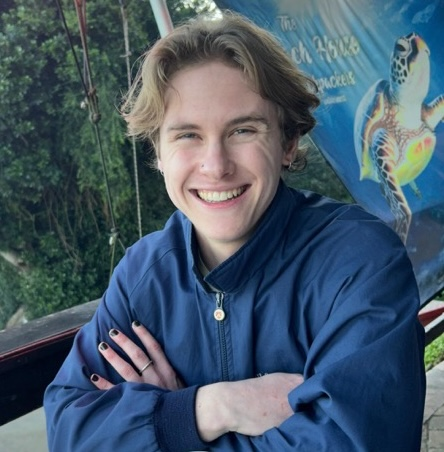
\includegraphics[width=2.8cm]{portrait.jpg}
\end{minipage}

\section{Education}

\textbf{Glenwood House} \hfill 2020 \\
National Senior Certificate

\textbf{Stellenbosch University} \hfill 2021 - 2025 \\
BSc Computer Science and Applied Mathematics

\textbf{Stellenbosch University} \hfill 2026 \\
BSc Honours in Computer Science

\section{Experience}

\textbf{Lifeguard} - Gwaing \& Wilderness Beaches, Garden Route \hfill 2018 - 2021 \\
Beach safety and emergency response across two surf beach postings.

\textbf{Waiter} - Dorp Bar, Stellenbosch \hfill 2023 - 2025 \\
Customer service in a demanding and busy bar.

\textbf{Tutor} - Teach Me2 \hfill 2025 - present \\
High school tutor in mathematics and IT.

\textbf{Teaching Assistant} - Stellenbosch University \hfill 2026 \\
Demonstrator for Software Engineering 344. Mark tutorials and project.

\section{Honours Year}
\subsection*{Thesis}
A teaching tool for Interferometry. A space science concept and technique used to capture celestial sources in 
the radio frequency realm. Using Earth aperture synthesis and stitching together the results from an array of radio telescopes, celestial sources 
can be are captured in great detail. The goal of this project was pedagogical and software orientated.

\subsection*{Course Work}

Functional Programming, Artificial Intelligence (Swarm Intelligence) and Computing and Society. \newline
Space Science algorithms, Principles of Data Science and Computer Vision.


\section{Projects}
\textbf{Optimise MeerKAT16 uv coverage} \hfill \href{https://github.com/Jordy-Ward/optimise-uv-coverage-using-GA}{github.com/Jordy-Ward/uv-coverage} \\
A comparative study into comparing heuristic Genetic Algorithms vs Simulated Annealing for finding optimal uv coverage for 16 MeerKAT antennas. 

\textbf{Large Scale Optimisation benchmark} \hfill \href{https://github.com/Jordy-Ward/LSOP-approaches-benchmarked}{github.com/Jordy-Ward/LSOPS-benchmark} \\
Implementing a stochastic scaling and subspace initialisation hybrid large scale optimisation algorithm and studying its effectiveness. 

\textbf{Differential Evolution} \hfill \href{https://github.com/Jordy-Ward/Differential-Evolution}{github.com/Jordy-Ward/Differential-Evolution} \\
Study of different cross over operators in differential evolution algorithms.

\textbf{Data School Hackathon 2026} \hfill Stellenbosch University \\
Ten day hackathon hosted by the School for Data Science and Computational Thinking and sponsored by Standard Bank.

\textbf{Prescient Coding Challenge 2025} \hfill \href{https://github.com/Jordy-Ward/prescient-coding-challenge-2025}{github.com/Jordy-Ward/prescient-coding-challenge-2025} \\
Data analysis solution presented by team DualBoot at the Prescient Investment Management hackathon.

\section{Skills}

\begin{tabular}{@{} l l}
  \textbf{Languages}  & Java, Python, JavaScript, C, Haskell \\
  \textbf{Frameworks} & React, Spring Boot \\
  \textbf{Tools}      & Git, PostgreSQL, LaTeX, Linux, MPI, OpenMP, REST API, Supabase, Neo4j \\

\end{tabular}

\end{document}
